\chapter{Vehicle}
Author: Florian Schwarzl

The DeepRacer itself represents a core part of this thesis, as it is used to test the trained models in a real-world environment. Our school acquired two of these cars. one of which we are using for this thesis. Below is a list of all parts delivered with one DeepRacer vehicle.

\begin{enumerate}
    \item Vehicle chassis
    \item Vehicle body cover
    \item Compute module battery
    \item Power cable and power adapter
    \item Vehicle battery
\end{enumerate}

The vehicle is separated into two parts. The upper part houses the compute-module and its battery. On top of the car are four small contraptions for holding the cove in place. The cover is a simple plastic sheet meant to serve as visual cover. This hood serves only the purpose of hiding the motor. Therefor we removed it during most of our training sessions. Metal clips are used to keep the cover in place during training.

\section{Chassis and Accessories}
The vehicle itself consists primarily of a four wheel drive chassis which holds all other components. The chassis can be further separated into a lower part, which contains the brushed electric motor, and an upper part that carries the compute module and a power bank to supply it. The entire car is build on a scale of 1/18 to a real car, meaning proportions like distance between wheels are realistic. This is especially apparent while driving, as one would expect better manoeuvrability and smaller turning radius.\repeatfootcite[p. 77]{AWS19}

At the front there are three USB ports used to mount the camera and other equipment like keyboards. As a crucial part of any self-driving car, the camera provided with the DeepRacer provides a 4-megapixel image, which is sent to the compute module. Since we are working with the first edition of the DeepRacer vehicle and not with the newer DeepRacer Evo, which has stereo cameras and a Light detection and ranging (LiDAR) sensor, obstacle avoidance and head-to-head racing are not supported by default. It is however possible to purchase an upgrade kit for 249,00 US\$, which includes an additional stereo camera and the LiDAR sensor.

\begin{figure}
    \centering
    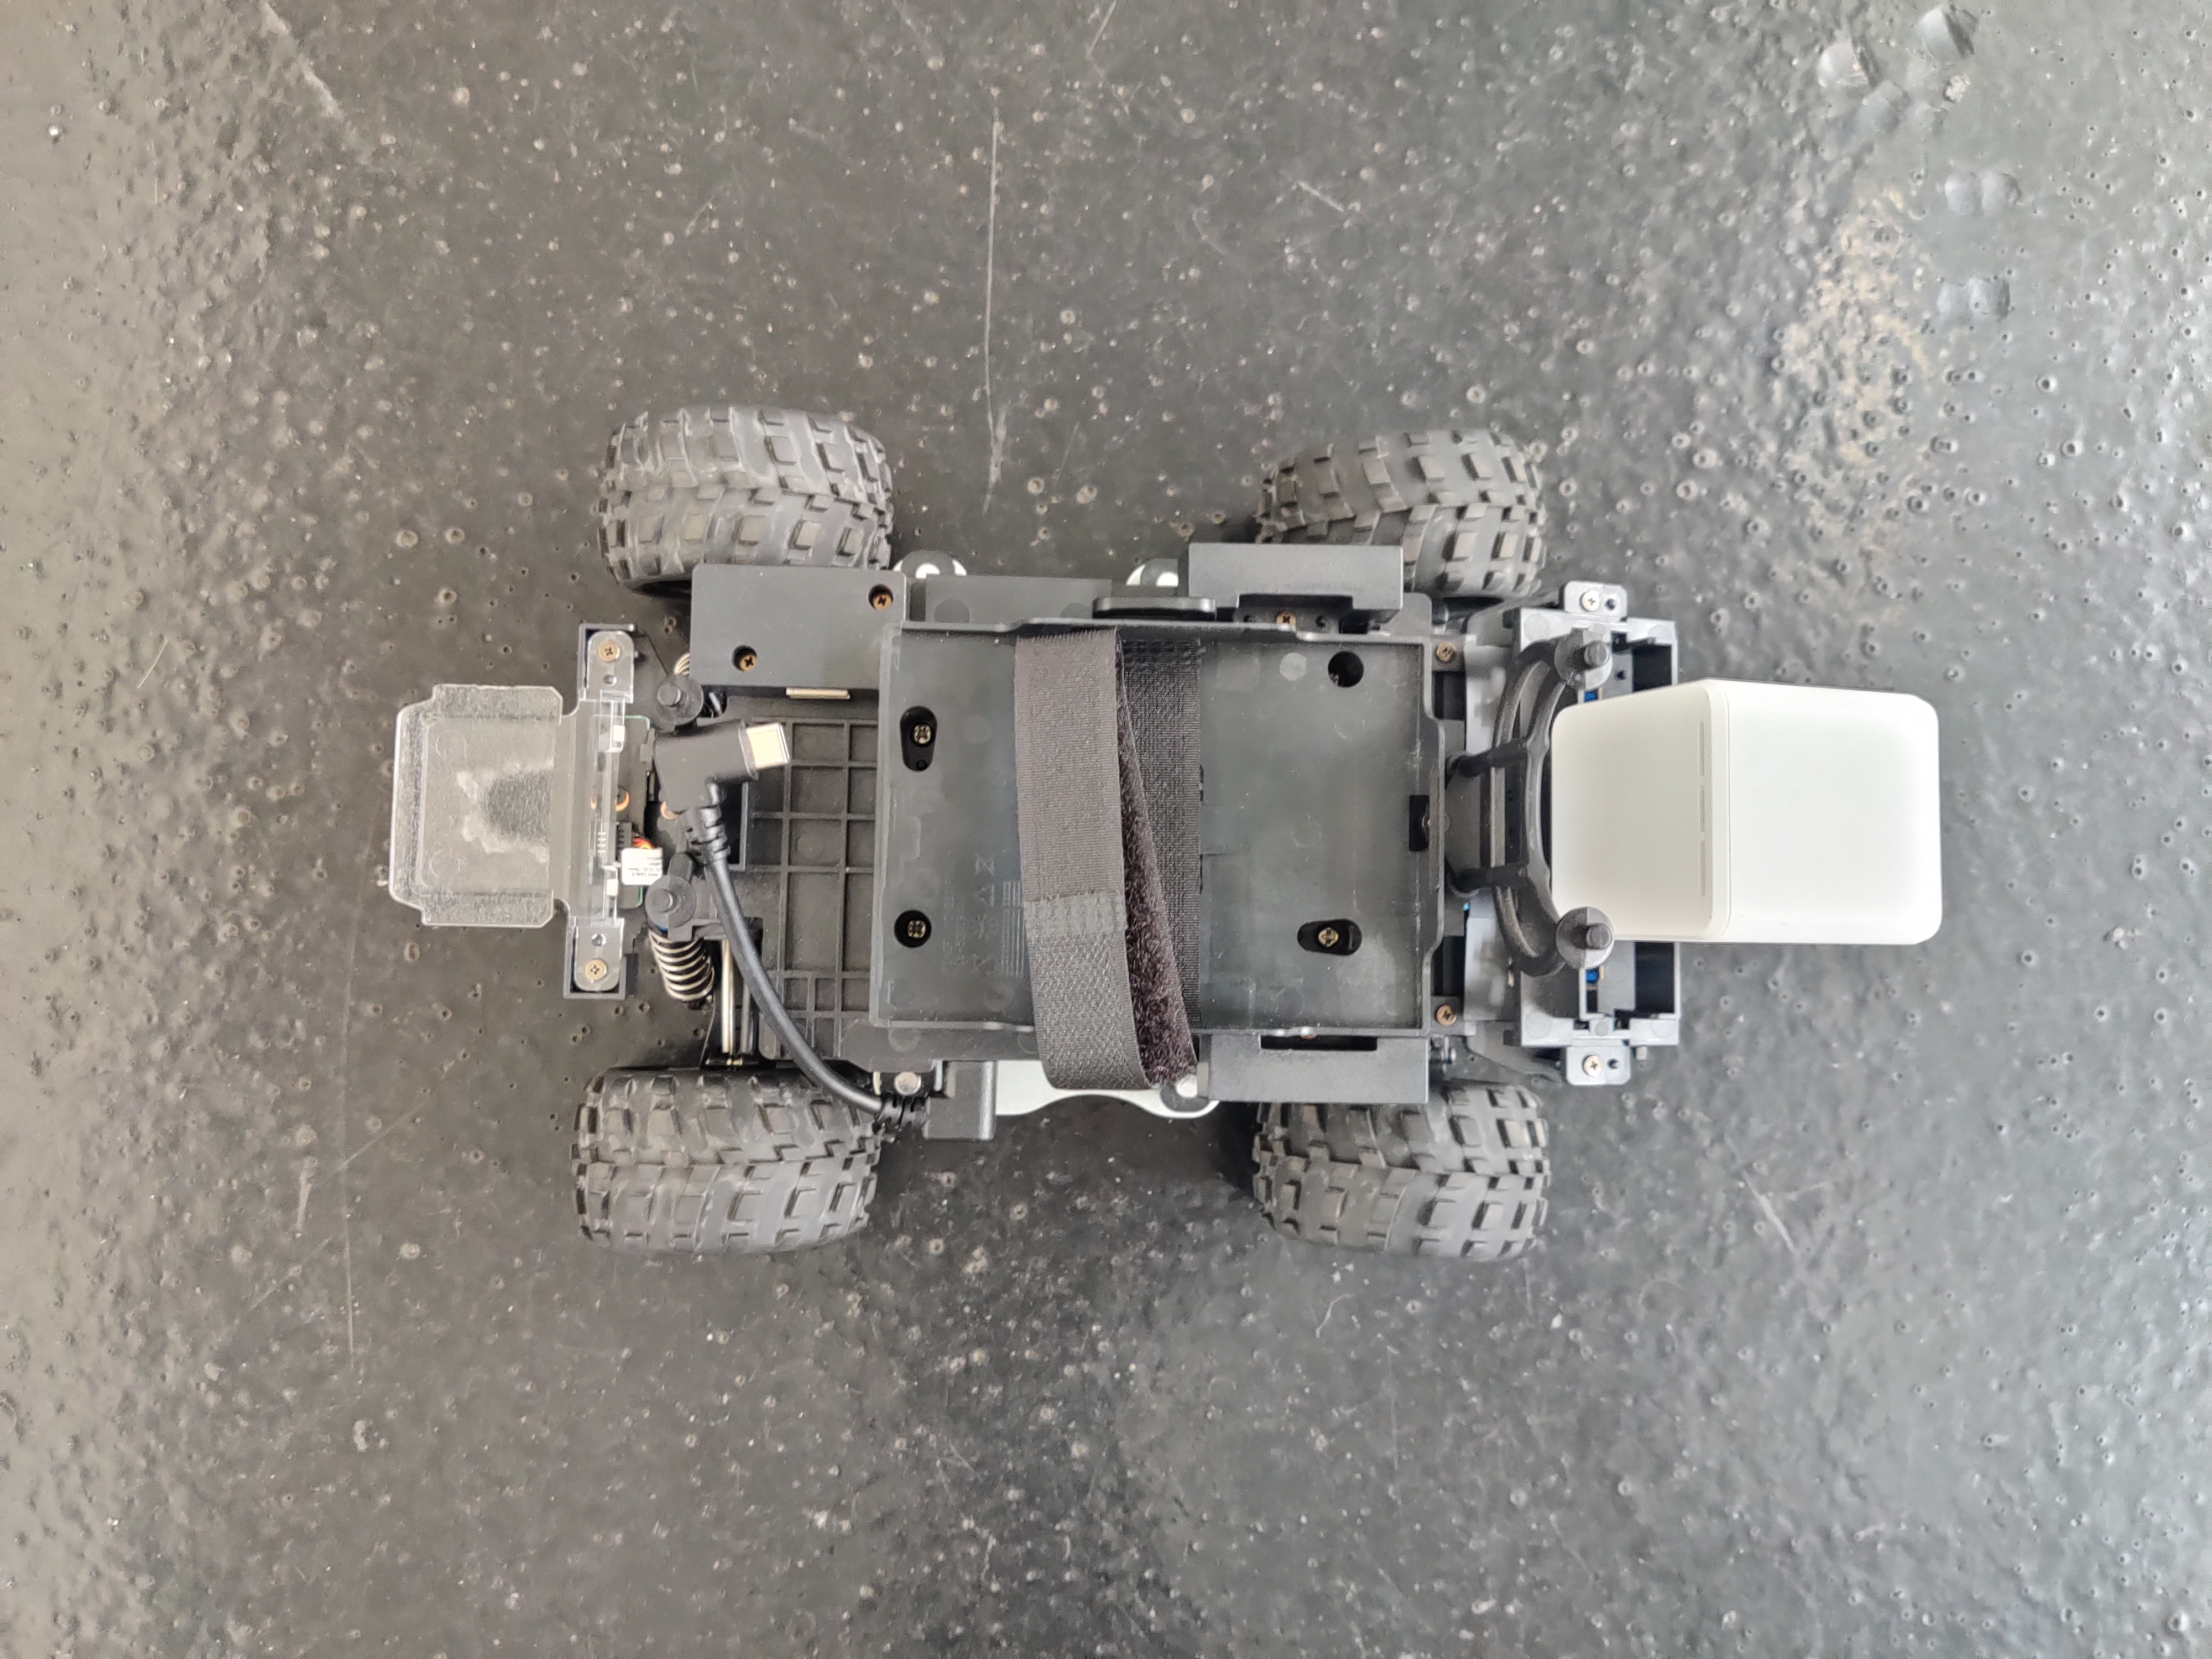
\includegraphics[width=.85\textwidth]{images/car_top_view.jpg}
    \caption{AWS DeepRacer Vehicle top view}
    \label{fig:vehicle_front}
\end{figure}

\subsection{Vehicle Steering}
The car an Ackermann front-wheel steering. The front wheels are mounted on suspensions which are connected with a second axis. This second axis, located behind the primary one is moved to the left or right and the wheels follow this movement. The steering pivots point inwards on the back of the front axle. They are connected via a bar called "track rod". By moving this bar to the left or right, the vehicles wheels are turned. The length of the track rod is slightly shorter than that of the axle. This leads to the wheels seemingly being misaligned, but this condition is intended.\repeatfootcite[p. 63]{Ackermann06}

\subsubsection{Advantage of Ackermann Steering}
The purpose of this steering mechanism is to minimize or in the best case completely eliminate wheel slip. The wheel alignment around a common turning point for both front wheels enables them to trace circles with different radii. Put differently, since the front wheels have different distances to the centre of the curve, in order to properly follow the intended path, they must turn at different angles.
% Include figure of Ackermann steering here

\subsubsection{Steering angle configuration}
The value which the agent uses as centre steering angle as well as the maximum steering angles can be configured via the web interface. This is necessary so that the car can drive in a straight line. Incorrectly configured steering can lead to severe hits in performance as the model has to compensate the drift caused by the misaligned wheels. In order to achieve the best results, the values defined in the action space before training should match the actions possible in real world scenarios. Alternatively, the steering configuration can be customised to fit the one defined in the action space. While fitting the simulation to the real world actions is likely to yield better results, it is often simpler to approximately configure the car's steering angle to match those defined in the action space.\repeatfootcite[p. 96]{AWS19}

\subsection{Vehicle and Compute-Module Batteries}
These batteries provide all parts with their necessary power. The battery supplying the compute-module is a common power bank with an USB-C connection. The one contained in the delivery provides 10 000 mAh of power. This is sufficient for operating it 3 to 4 hours. 

The second battery which powers steering and engine has less capacity and smaller in dimension. Its capacity is 7 500 mAh, which is enough for about 1 hours of continuous driving.

Replacements are confortable with ease, as both are easily accessible and replacement parts can be ordered online at reasonable prices. Especially the power bank used for the compute-module does not have to meet any other criteria than to fit on top of the vehicle and have sufficient capacity.

\section{Compute Module}
The upper component houses the ``brain'' of the car. The compute module consists of an Intel Atom
%todo: Fix trademark symbol
processor, 4 Gigabyte of RAM and 32 Gigabyte memory, which can be expanded via a SD card. This hardware is running Linux Ubuntu 16.04.3 with Intel OpenVINO\texttrademark{} and ROS\footnote{Robot Operating System} Kinetic. Apart from that the chassis offers 4 USB type A ports, 1 USB type C port, 1 Micro-USB port and one HDMI port. The USB type C port is used to supply the compute module with power, while the HDMI port offers the ability to connect a display and directly access the modules operating system.

As seen in figure \ref{fig:vehicle_front}, facing the left side of the car are three small LED lights. These lights are used to display the status of the power supply and the wireless LAN-connection. The first light indicates various states of the compute module, more precisely the states of the operating system running on the compute module. The following list shows the possible stages that this indicator can display.\repeatfootcite[p. 82 f.]{AWS19}
\begin{itemize}
    \item \textbf{Off} signals that the computer is turned off or is not supplied with sufficient power.
    \item \textbf{Blinking yellow} indicates the BIOS and the operating system being loaded after pressing the power button.
    \item \textbf{Steady yellow} means that the operating system is loaded and ready to use in a short amount of time.
    \item \textbf{Steady blue} shows that there is currently an application running on the compute module. This  light is also on while automated driving is activated.
    \item \textbf{Blinking blue} indicated that a software update is in progress.
    \item \textbf{Steady red} signals that an error occurred either during startup or while running an application.
\end{itemize}

\begin{figure}
    \centering
    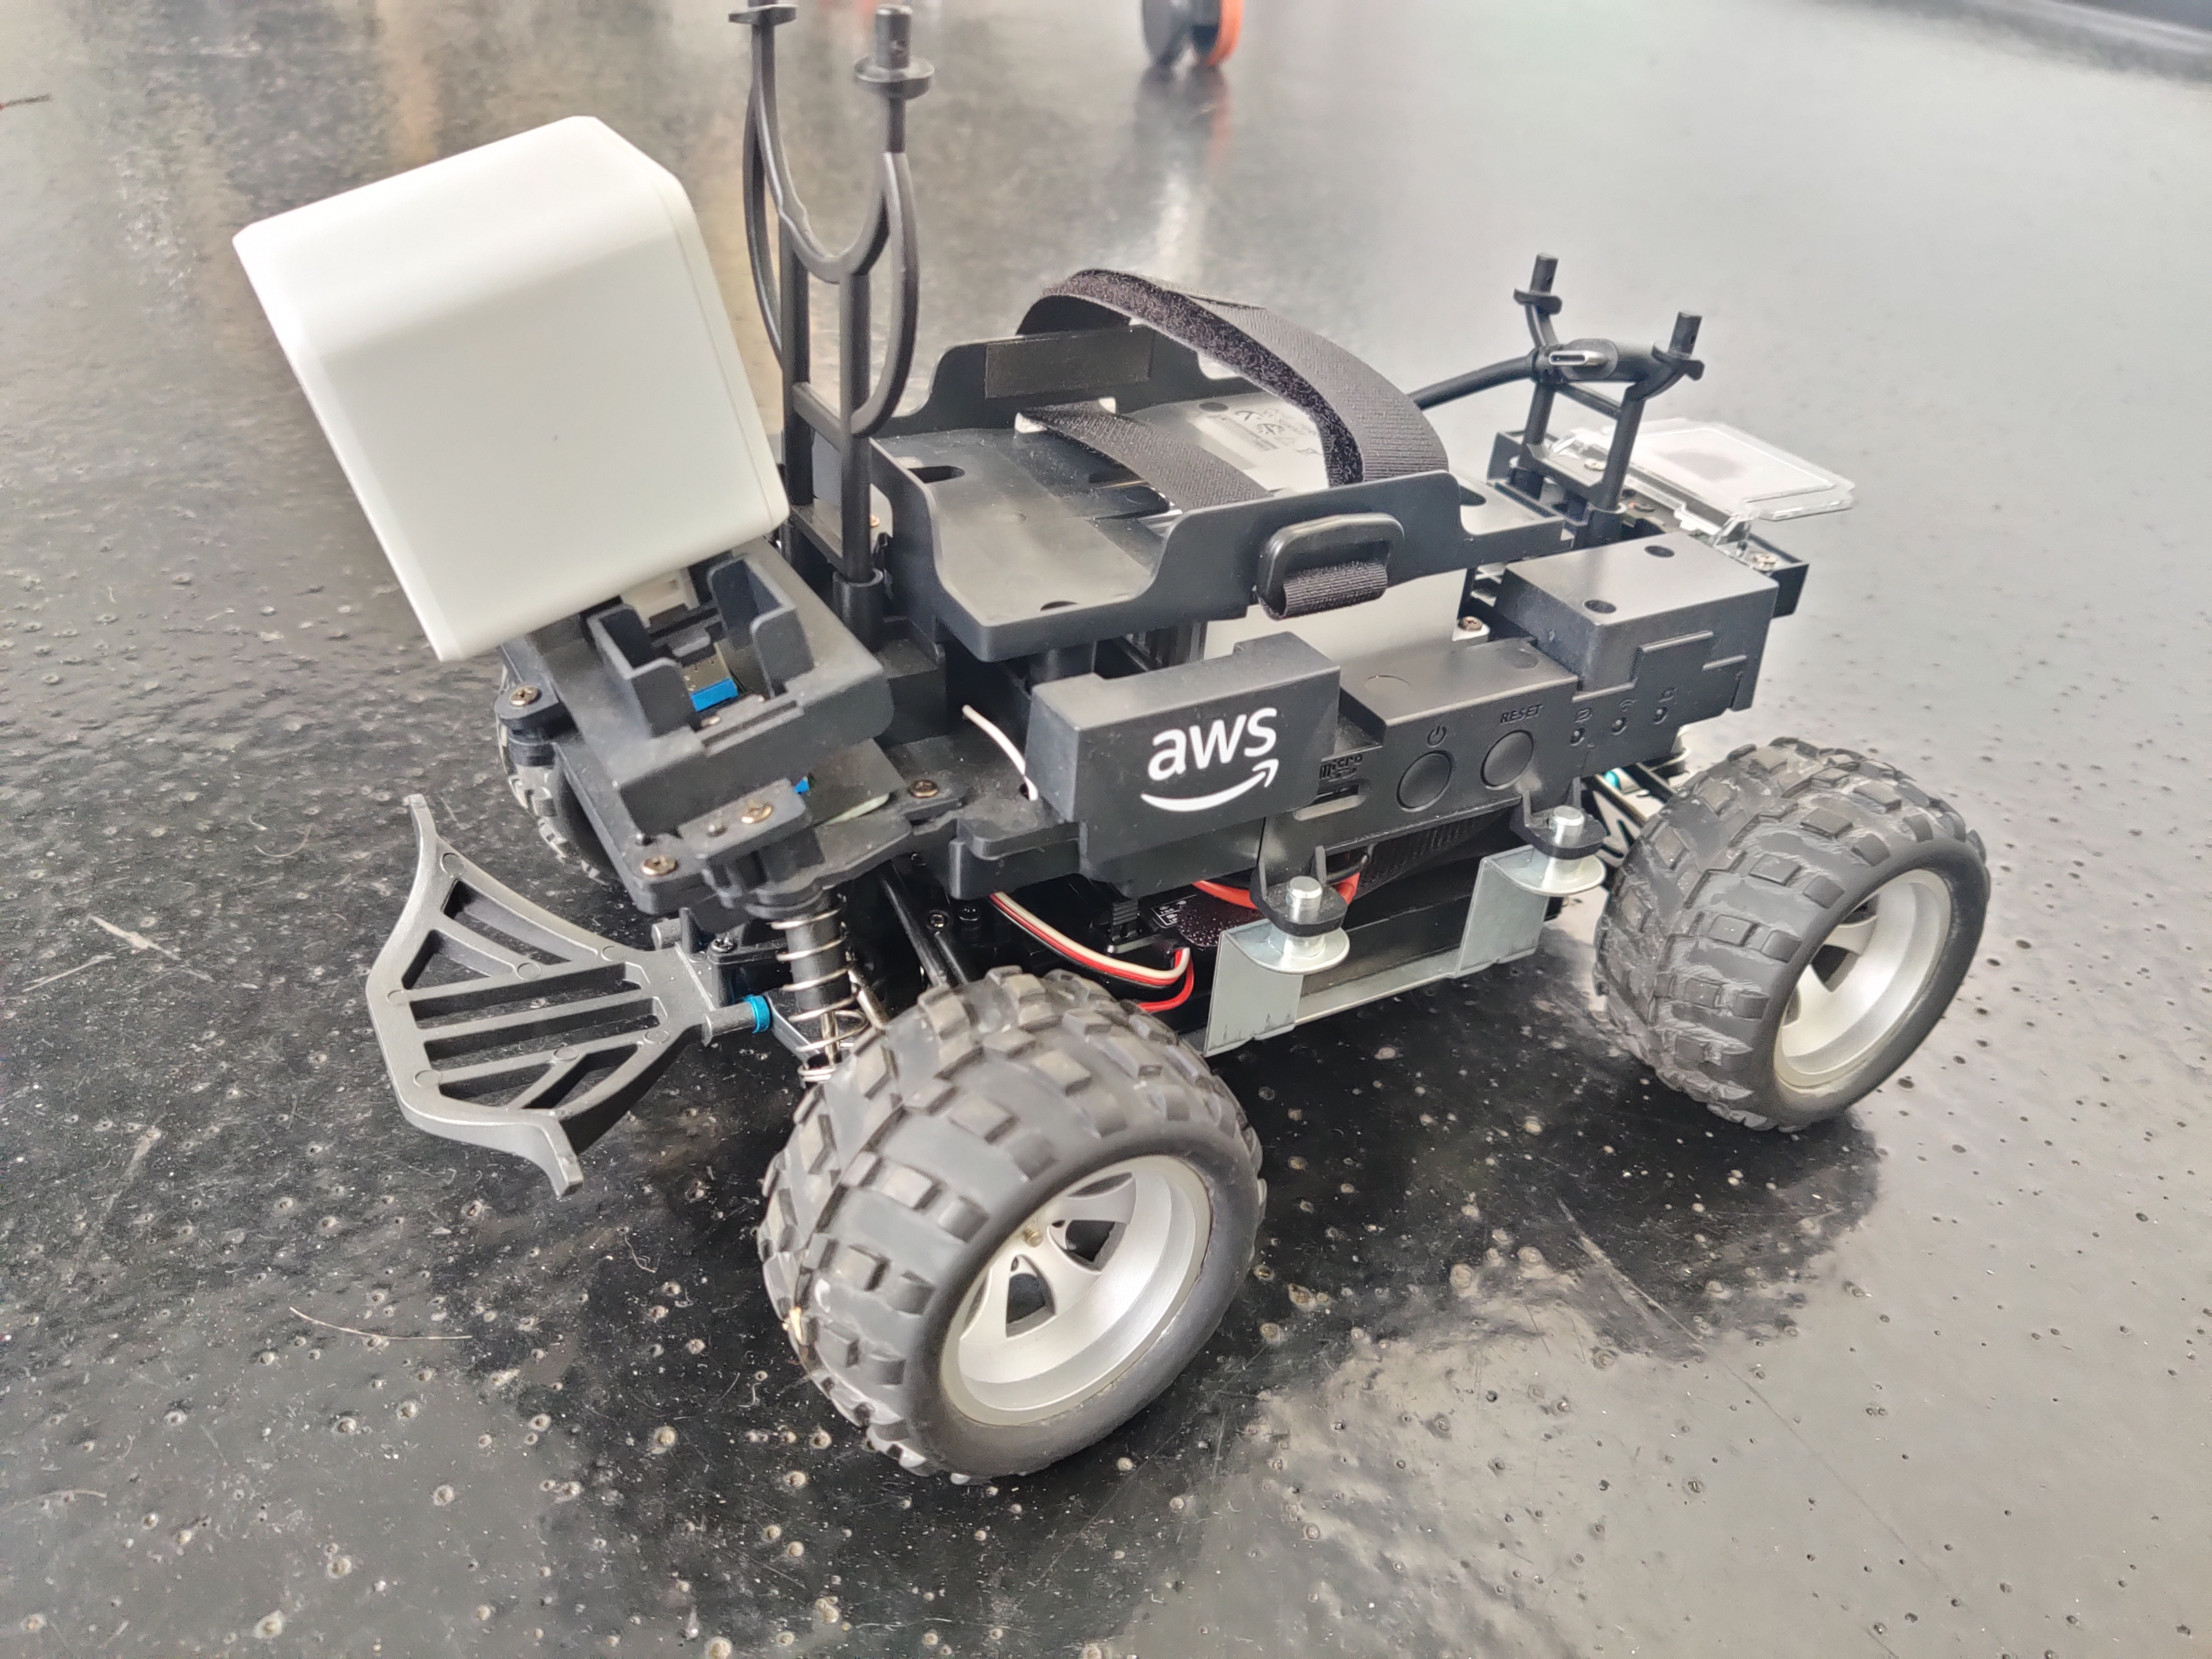
\includegraphics[width=.85\textwidth]{images/IMG_20201117_091128.jpg}
    \caption{AWS DeepRacer Vehicle side view}
    \label{fig:vehicle_side}
\end{figure}

\subsubsection{Web-Interface}
The compute module hosts its own web interface, from which the vehicle can be monitored, remotely controlled and configured. This interface is meant to be the main access point when working with the car. The website can be retrieved by accessing the IP-address of the car with a web browser. The address as well as the password which are required in order to access the configuration interface can be found on a label on the bottom of the car. The primary purpose of the website is configuration. This is indeed very useful as it removes the need to access the compute modules operating system directly. Without the web-interface, for every change it would be necessary to directly access the operating system by connecting a display, mouse and keyboard.

\begin{figure}
    \centering
    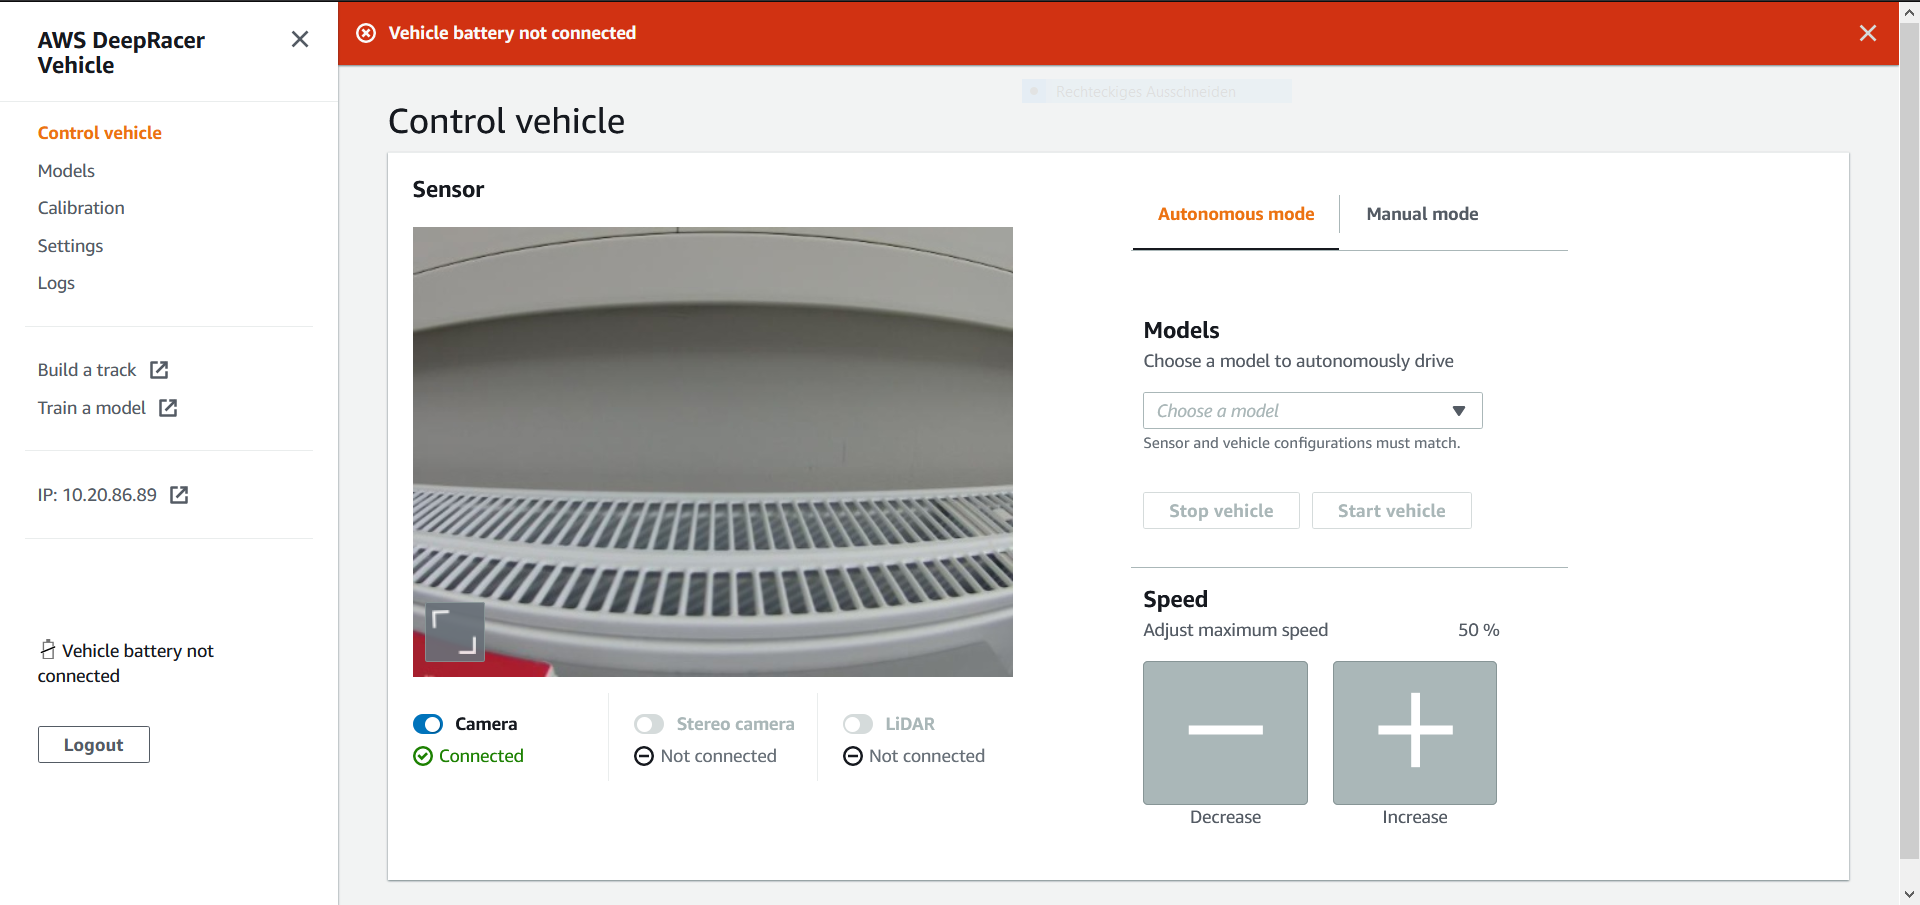
\includegraphics[width=.85\textwidth]{images/deepracer_console_1.png}
    \caption{DeepRacer Web interface}
    \label{fig:web_interface}
\end{figure}

\subsection{Configuration}
This section covers the configuration option possible via the web interface. There are two possible options that can be adjusted. The first one is the maximum and stopping speed. This setting determines how fast the car will drive when speed is set to maximum. The stopping speed sets the minimum power which the motor receives.

\subsection{Sensors}
In order to acquire the necessary information from the environment, the agent is outfitted with at least one sensor. Although we are only using the camera provided as a default sensor, this subsection covers other sensors available.

As mentioned, the default sensor provided is a single front-facing camera, connected via an USB-port at the front of the vehicle. The image provided by this part is the only information which the agent receives from its environment. This information is sufficient for the agent to traverse a marked track without obstacles or other vehicles. The only other information at our disposal is the sensor data from the electric motor and steering control. This provides us with information about the current speed and steering angle. Apart from that, all other information comes solely from the camera. Considering this, it is impressive that with a simple camera image, an entire vehicle can be controlled autonomously.

\section{Remote Control}
By default the DeepRacer vehicle offers the option for remote control via a virtual joystick on its web-interface. The direction as well as speed can be controlled this way. The input of this joystick is send to the car via an web-based application program interface (API). This API is hosted on the same web-server as the local interface seen in figure \ref{fig:web_interface}, this however shows the option for autonomous driving. Switching to manual control is done by selecting the manual mode tab located at the top right corner. After selecting the manual control tab, the website shows the joystick instead of the model selection menu. This can be seen in figure \ref{fig:manual_control}. Below the analogue-stick is the menu used for configuring the maximum speed. The current value is shown above the two buttons in percent. As an example, a value of 50 percent indicates that, when the analogue-stick is pressed all the way forward, the car drives at half of its highest possible velocity. This is the default way of remote controlling and sufficient enough for simple tests. If a more precise and ergonomic control mechanism is desired then it is necessary to directly access the underlying API. Accessing the  electric motor directly via ROS\footnote{Robot Operating System} is possible but not required. Driving this way has several disadvantages, most notably is it not possible to connect a game controller or similar device to the compute module, since the module does not have Bluetooth. Counteracting this can be achieved by using a computer as middle man. The game controller is connected to the computer, which sends the input to the vehicles manual control API.

\subsection{Web-API}
The application program interface is hosted on the same web-server as the rest of the local website. It is accessible behind the <IP-address>/api/ path. In order to access remote control, the correct credentials have to be put in and send to the /api/login endpoint. This then returns a session cookie which authorises the usage of other functionalities. The cookie has to sent with every request, otherwise it will return with an error stating an unauthorised access. The following list shows all endpoints relevant for remotely steering the car.

\begin{itemize}
    \item \textbf{Endpoint: start\_stop}: This API endpoint accepts the PUT method with a JSON-object with one field set. This field is named start\_stop and can take on either string of start or stop. It tells the car to either start or stop on the spot. This API call is required before beginning to drive.
    \item \textbf{Endpoint: manual\_drive}: Expects HTTP method PUT with a JSON-object containing the steering angle, speed and maximum speed.
\end{itemize}

The first API call is only used to start the car before driving. Without this, the vehicle will not move, even if told to do so by the second command. The endpoint manual\_drive is used to control the vehicle. It continuously receives requests which consist of three fields. The first field is named angle and defines the steering angle as a value ranging from -1 to 1. In this context, -1 is defined as a full left turn, while 1 represents a sharp right turn. The actual degree are set in the configuration menu under the maximum-steering-angle section. The second field is labeled throttle and represents the speed of the vehicle on percent. The percentage is taken from the maximum speed possible. A value of 0.5 is equal to half the maximum speed. The third field sets the maximum speed in metres per second. The actual speed can be calculated by multiplying the throttle field with the maximum speed.

\begin{figure}
    \centering
    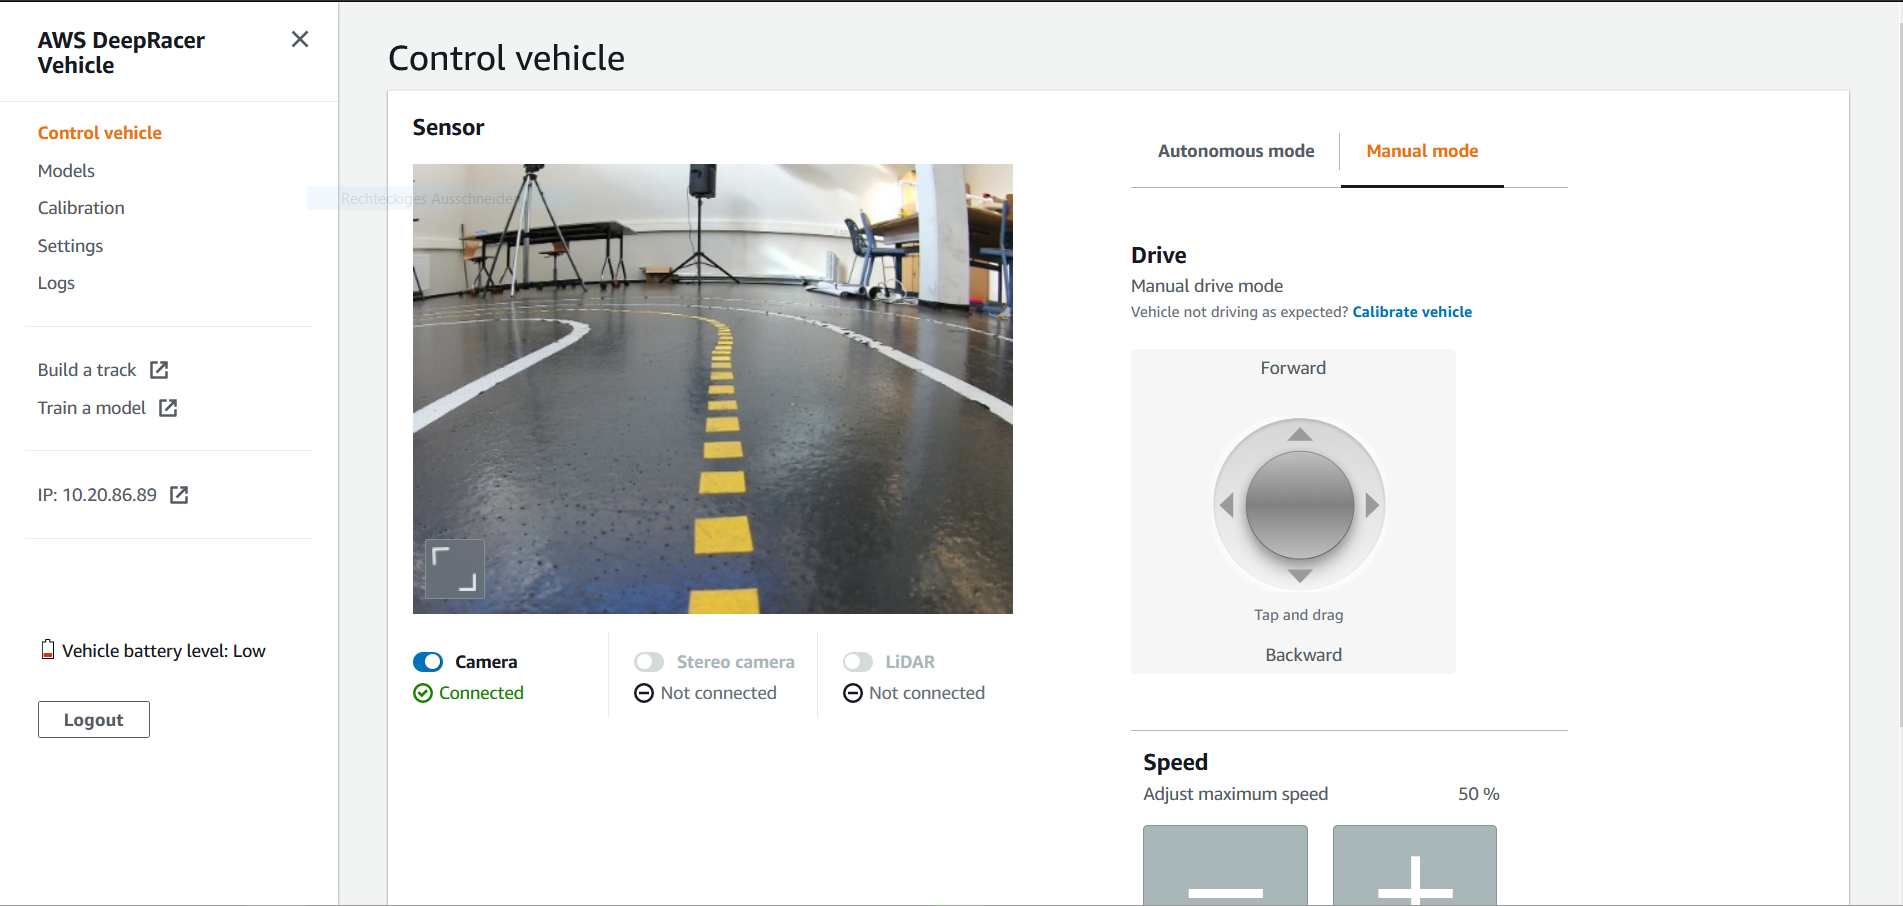
\includegraphics[width=.85\textwidth]{images/manual-control.png}
    \caption{Manual control interface}
    \label{fig:manual_control}
\end{figure}
